\section{基本介绍及安装方法}

本节将一步步展示如何安装配置本集成工具。

\begin{figure}[H]
    \Centering
    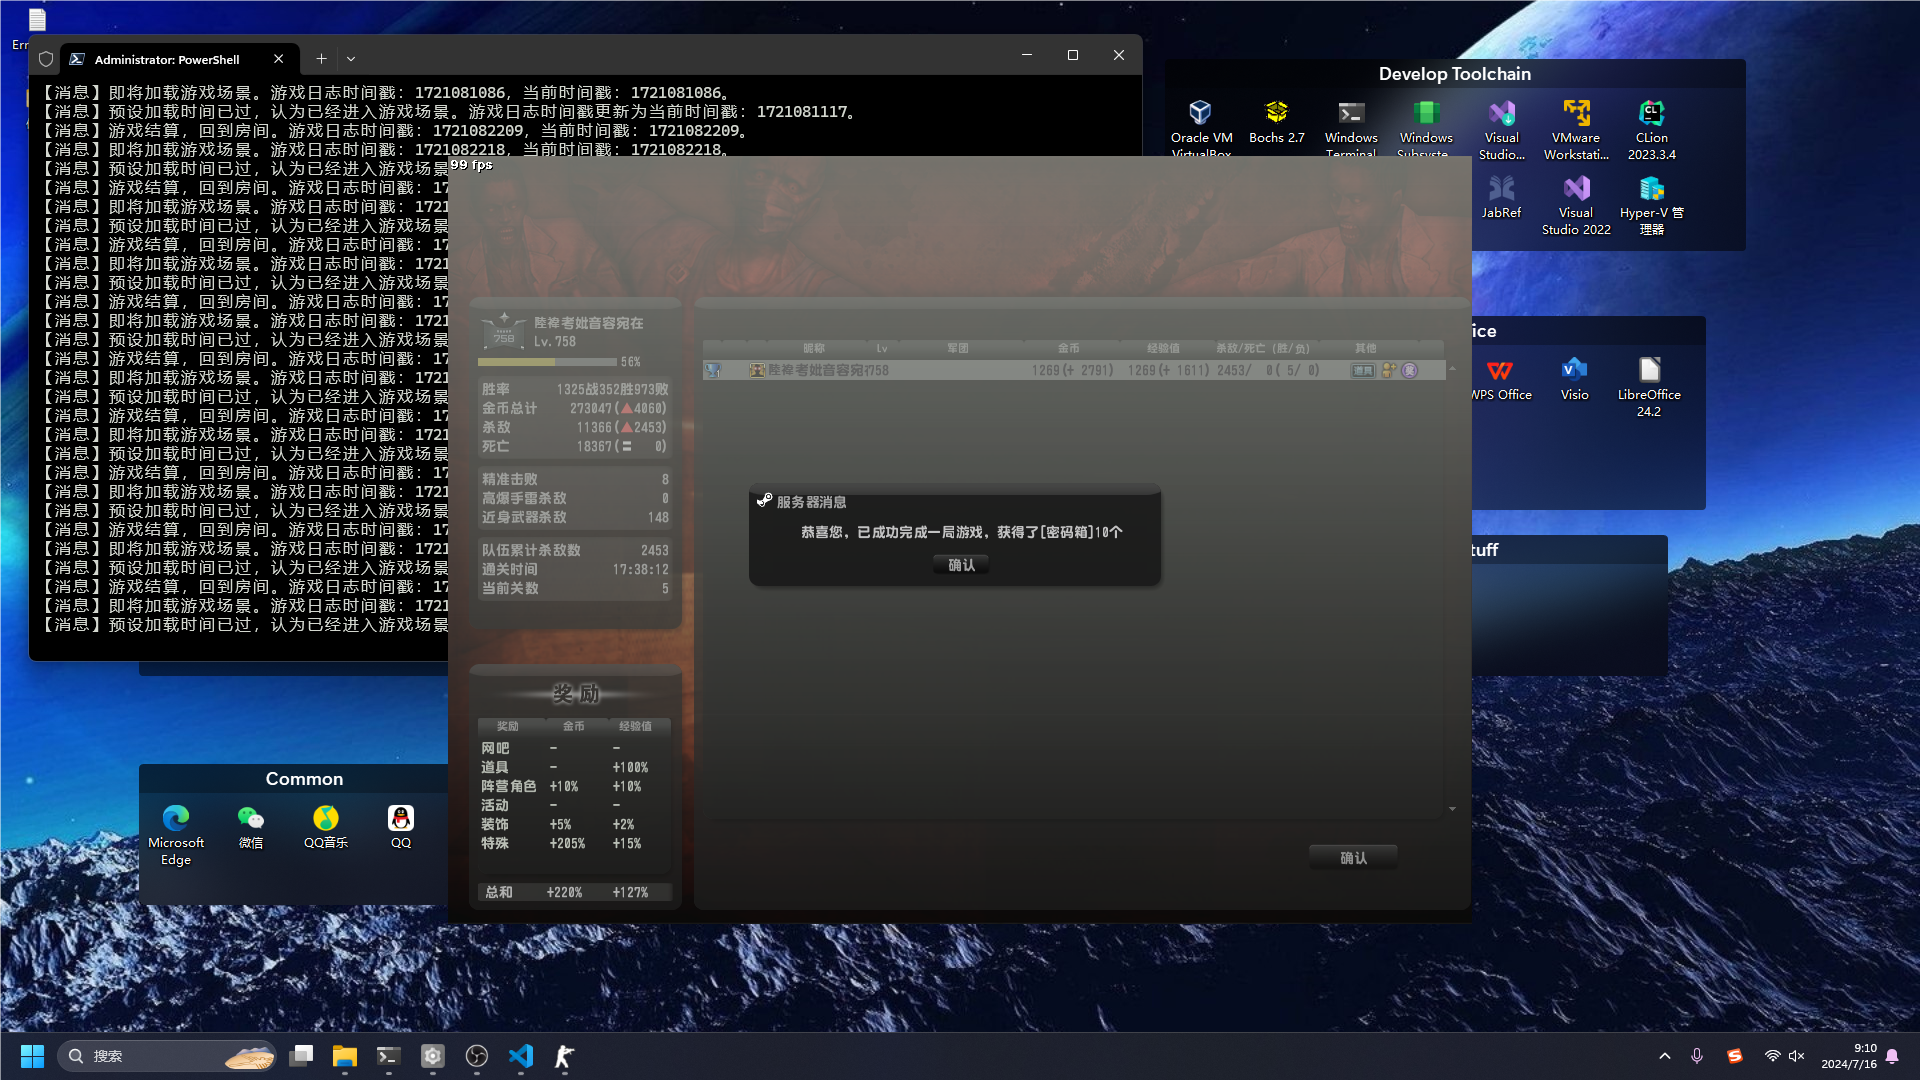
\includegraphics[width=\textwidth]{docs/assets/controller.png}
    \caption{运行效果展示}
\end{figure}

\subsection{开始之前}

\textbf{\color{red}Windows 会锁定从网络上下载得到的文件,这会导致 Powershell 文件无法运行,需先对下载得到的压缩包右键并点击“属性”,接着点击“解除锁定”,然后点击“确认”以解除锁定状态。如果压缩包未被锁定(没有“解除锁定”选项),可跳过此步骤。}

\begin{figure}[H]
    \Centering
    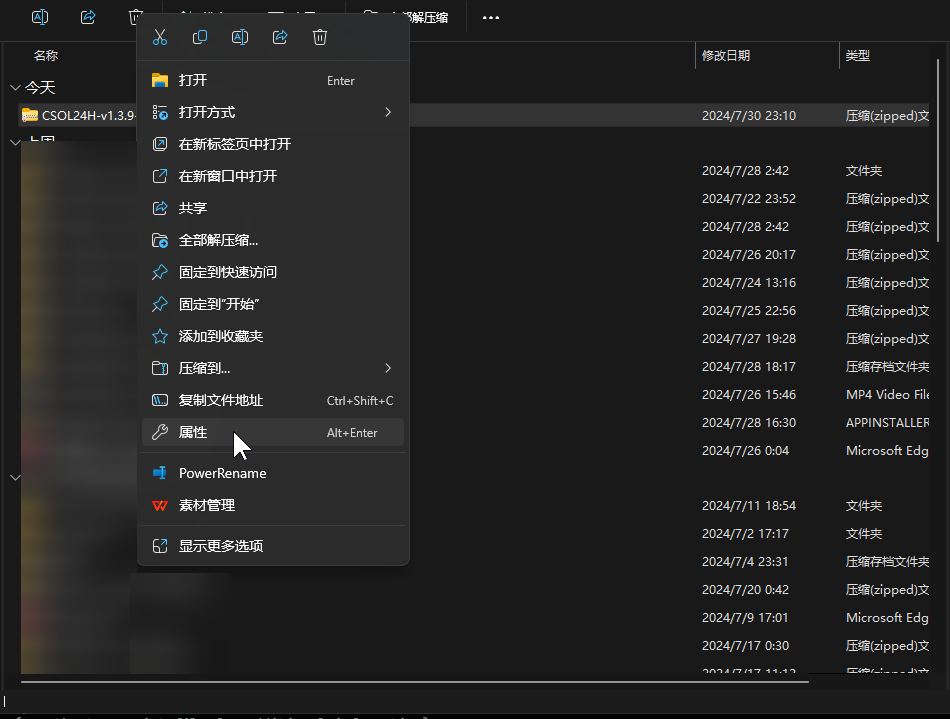
\includegraphics[width=\textwidth]{docs/assets/unlock_00.png}
    \caption{右键后在弹框中点击“属性”}
\end{figure}

\begin{figure}[H]
    \Centering
    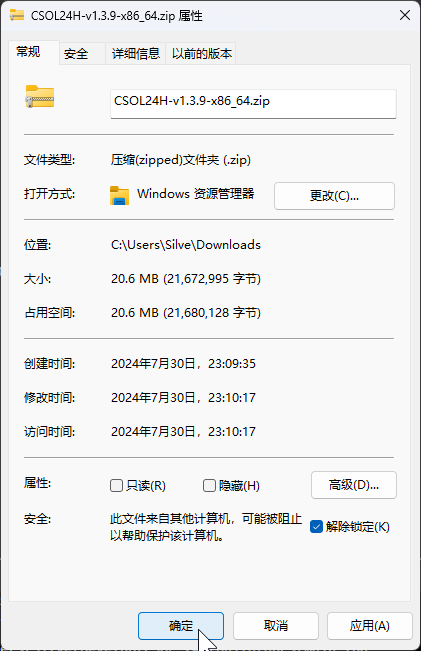
\includegraphics[width=\textwidth]{docs/assets/unlock_01.png}
    \caption{点击“解除锁定”并确认}
\end{figure}

将解除锁定后的压缩包解压。\textbf{\color{red}注意,解压路径不能包含非英文字符},否则 LUA 脚本无法运行。

\textbf{\color{red}注意,Windows 文件系统不区分文件名的大小写,因此,若您在接下来的步骤中遇到名称相同但大小写不同的文件名,应将其视为完全一样的文件名。}

Windows 默认情况下严格阻止运行任何 Powershell 脚本文件(后缀为 \lstinline{.ps1}),因此若您是第一次使用本工具,需要做如下配置。

对于 Windows 11 23H2 及以上版本的用户:打开“设置”,点击“系统”-“开发者选项”,在“Powershell”下拉选项中打开图示选项即可。下面针对 Windows 11 23H2 以下版本用户的设置步骤可忽略。

对于 Windows 11 23H2 以下版本的用户,按下 \lstinline{Win} \lstinline{R},输入 \lstinline{powershell} 后,按下 \lstinline{Ctrl} \lstinline{Shift} \lstinline{Enter} 以管理员权限打开 Powershell 窗口。

\begin{figure}[H]
    \Centering
    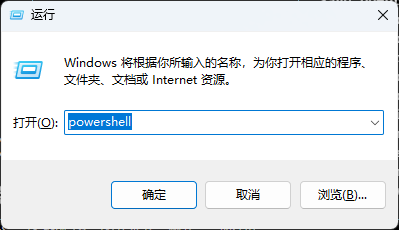
\includegraphics[width=\textwidth]{docs/assets/run_pwsh_as_admin.png}
    \caption{在“运行”中输入 \lstinline{powershell},并按 \lstinline{Ctrl} \lstinline{Shift} \lstinline{Enter}}
\end{figure}

输入下面的命令:

\begin{minted}{powershell}
Set-ExecutionPolicy -Scope CurrentUser -ExecutionPolicy RemoteSigned
\end{minted}

然后,回车运行上述命令,过程中可能需要您输入“Y”确认。运行完成后即可关闭窗口。

\begin{figure}[H]
    \Centering
    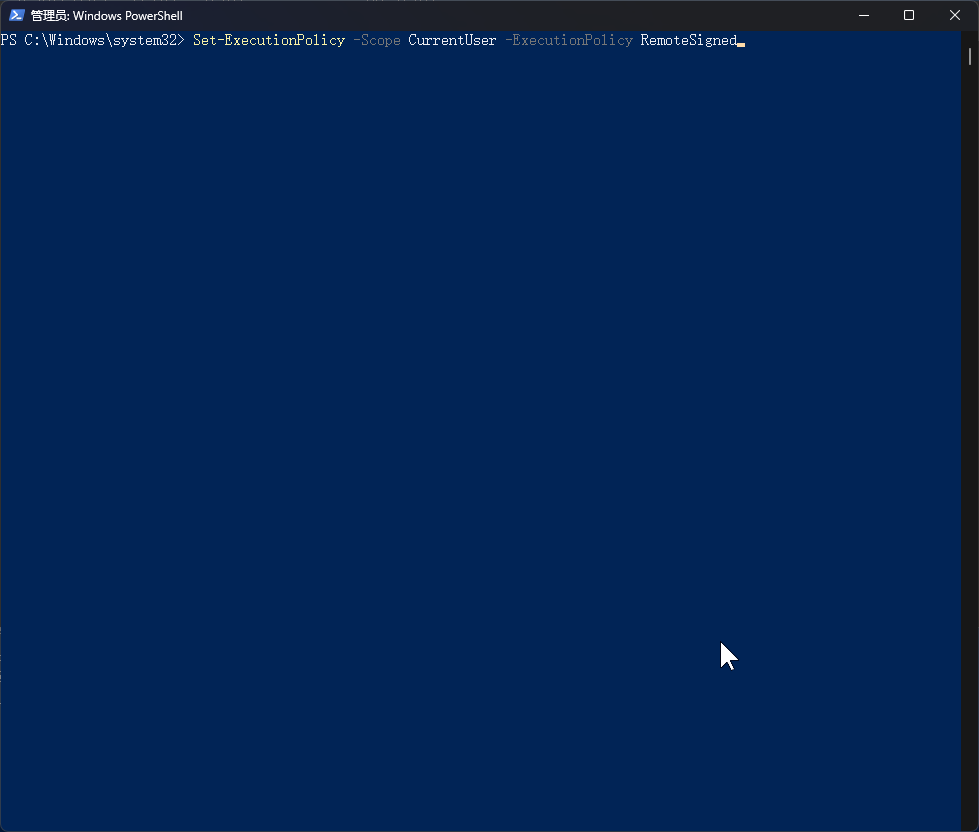
\includegraphics[width=\textwidth]{docs/assets/confirm_execution_policy_00.png}
    \caption{键入修改执行策略的命令}
\end{figure}

\begin{figure}[H]
    \Centering
    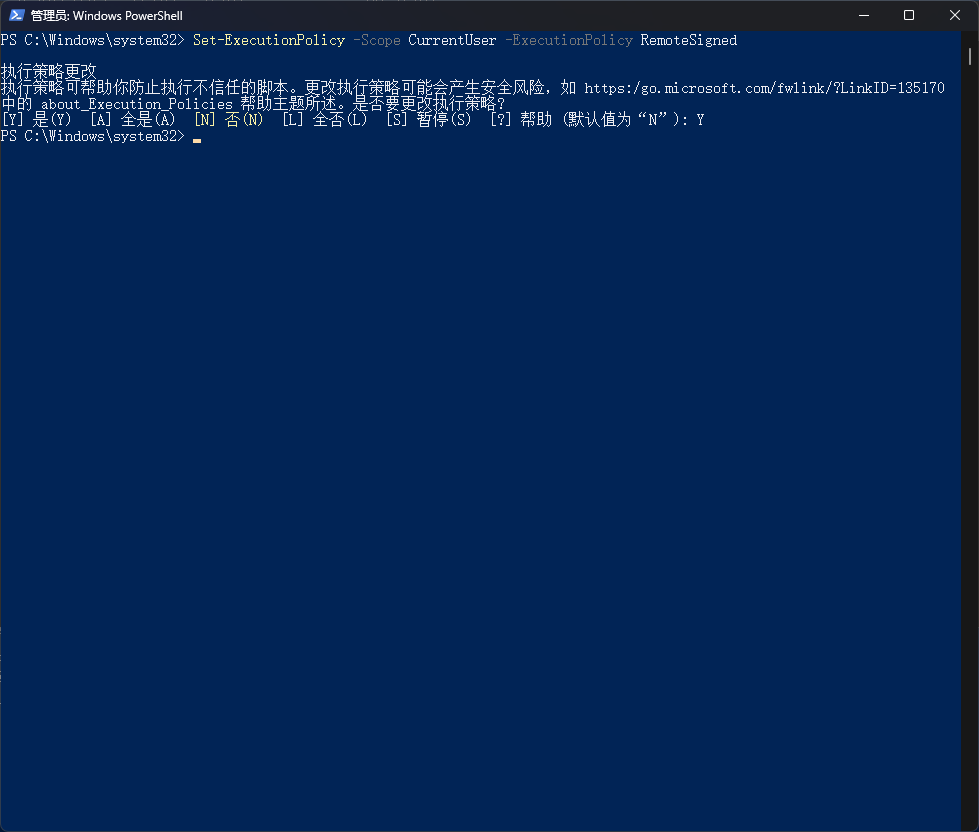
\includegraphics[width=\textwidth]{docs/assets/confirm_execution_policy_01.png}
    \caption{确认修改执行策略}
\end{figure}

\subsection{罗技软件导入 LUA 程序}

鼠标右键点击集成工具文件夹中的 \lstinline{install.ps1},点击在 Powershell 中运行,完成对 LUA 主程序 \lstinline{Main.lua} 的配置。

\textbf{\color{red}配置完成后,如果变动了安装路径(移动集成工具文件夹或将集成工具文件夹重命名),则需要重新运行一次 \lstinline{install.ps1},并重新在罗技软件中保存并运行(详见下文)。}

\begin{figure}[H]
    \Centering
    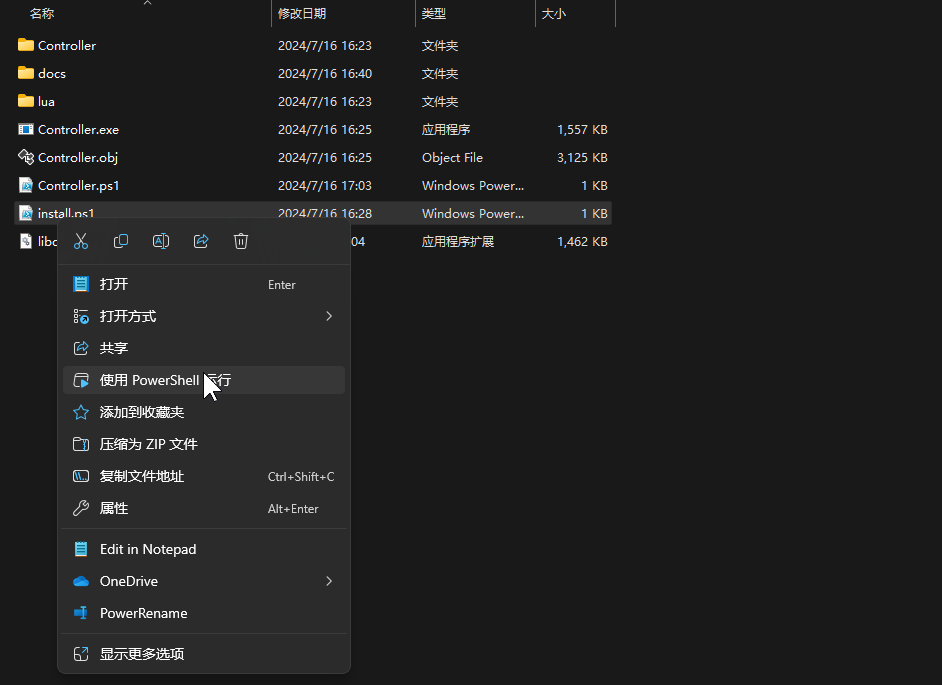
\includegraphics[width=\textwidth]{docs/assets/install.png}
    \caption{运行 \lstinline{install.ps1}}
\end{figure}

然后,前往罗技官网下载安装最新版的 Logitech G HUB 软件(以下简称为“罗技软件”)。\textbf{\color{red}本集成工具并不需要您拥有任何的罗技硬件设备。}

安装并\textbf{\color{red}以管理员权限}启动 Logitech G HUB 软件。否则会因为权限问题导致游戏无法正确接收软件发出的键鼠消息。

\begin{figure}[H]
    \Centering
    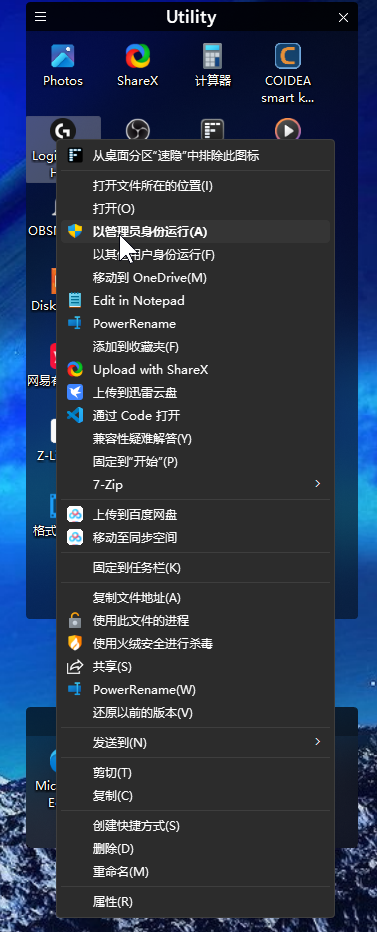
\includegraphics[width=\textwidth]{docs/assets/run_lghub.png}
    \caption{以管理员权限运行 Logitech G HUB}
\end{figure}

\textbf{\color{red}当已经存在罗技软件进程时,运行罗技软件不会再启动新的实例,新打开的进程将会退出以保留旧进程。因此,当存在正以普通权限运行的罗技软件进程时,以管理员权限启动罗技软件是无效的。故在以管理员权限启动罗技软件前,请务必确保罗技软件相关进程处于关闭状态。}
确认方法为:打开任务管理器,搜索 “logi”,结束\textbf{\color{red}除“Logitech Updater”(罗技软件更新守护进程,无需关闭)}以外的所有与罗技软件相关的进程(参考下图)。

\begin{figure}[H]
    \Centering
    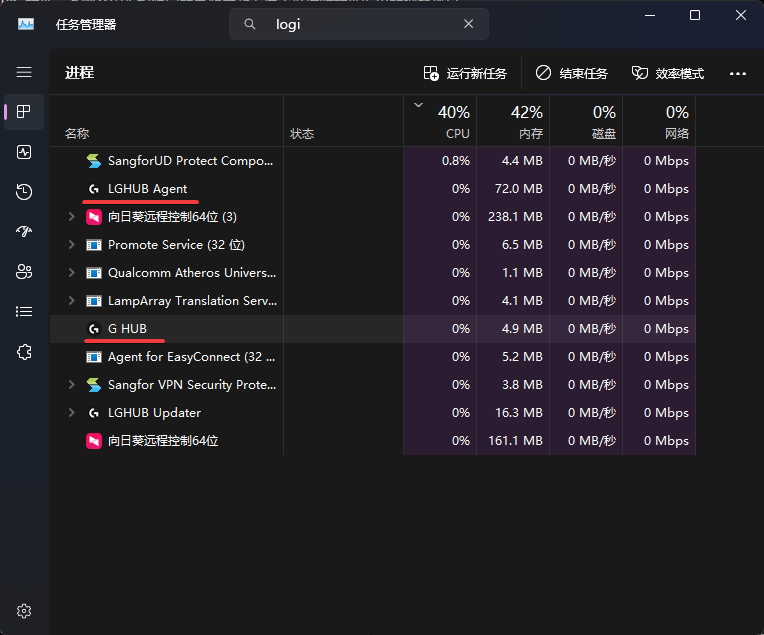
\includegraphics[width=\textwidth]{docs/assets/search_lghub_process.png}
    \caption{搜索罗技软件进程}
\end{figure}

然后,将这些进程全部结束。

\begin{figure}[H]
    \Centering
    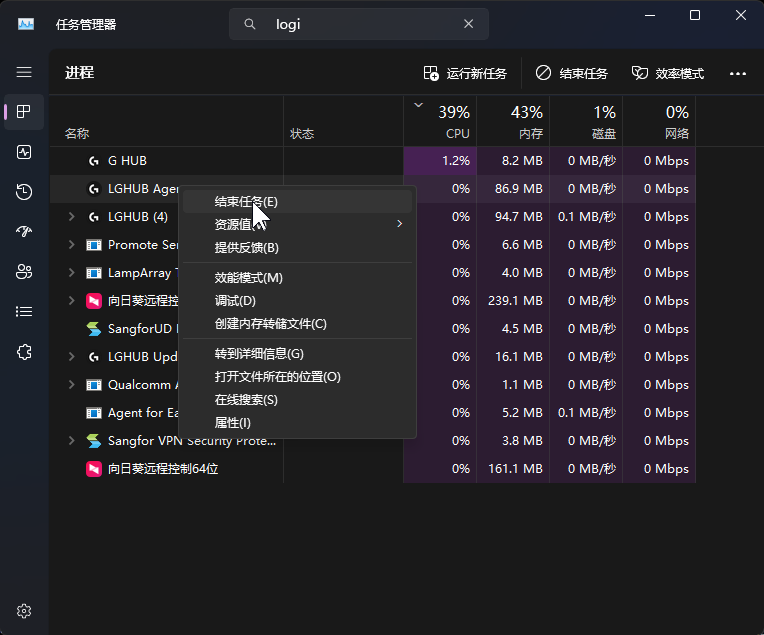
\includegraphics[width=\textwidth]{docs/assets/terminate_lghub_00.png}
    \caption{结束罗技软件进程}
\end{figure}

\begin{figure}[H]
    \Centering
    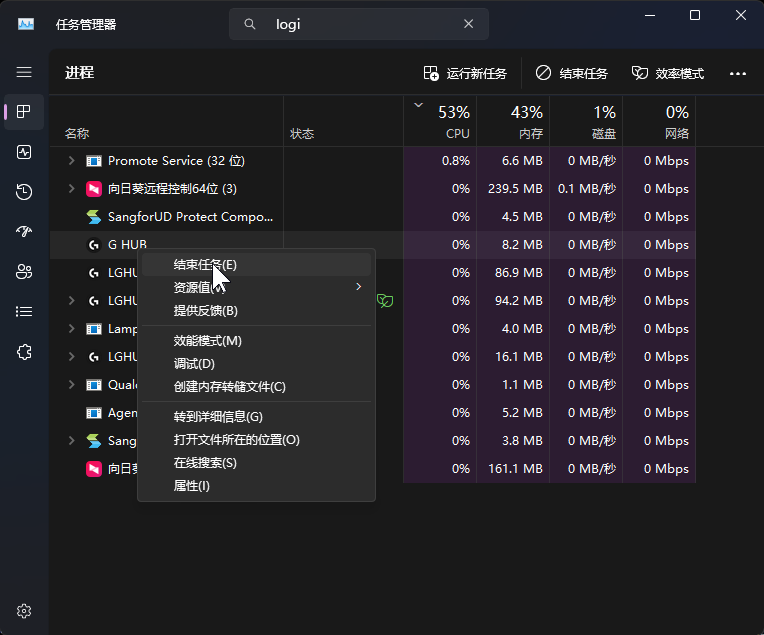
\includegraphics[width=\textwidth]{docs/assets/terminate_lghub_01.png}
    \caption{结束罗技软件进程}
\end{figure}

上述操作完成后,进入罗技软件主界面。

\begin{figure}[H]
    \Centering
    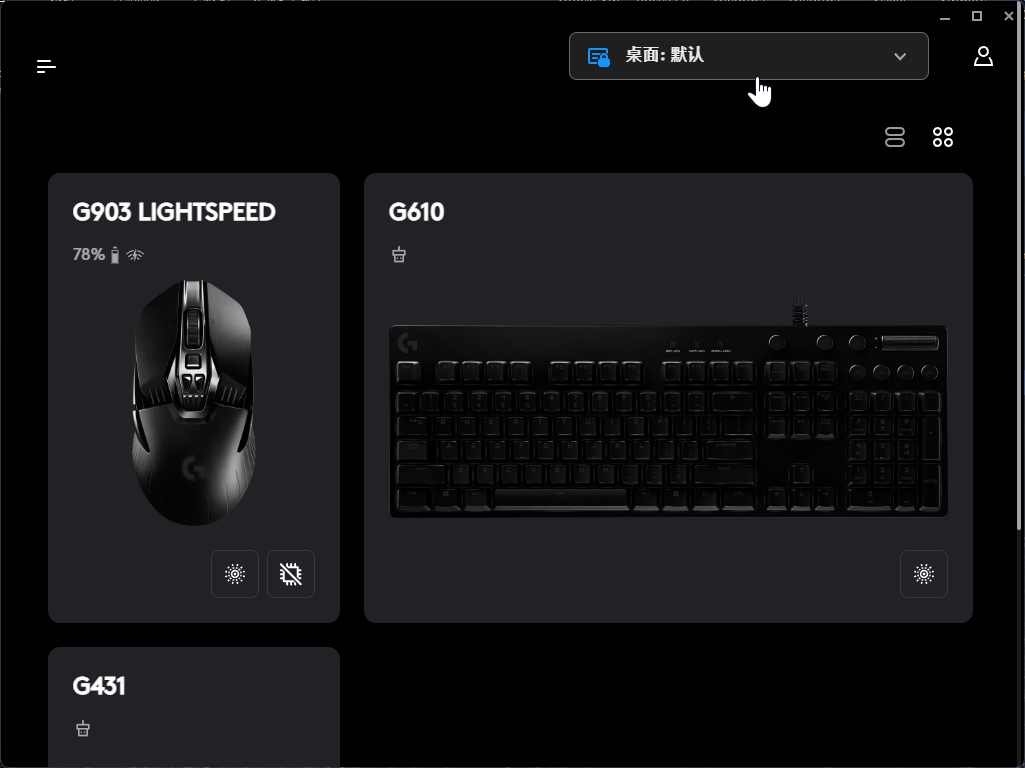
\includegraphics[width=\textwidth]{docs/assets/lghub.png}
    \caption{罗技软件主界面}
\end{figure}

点击左上角展开菜单后再点击“设置”。在设置界面中关闭软件开机自启,防止软件以普通权限自启(设置软件以管理员权限开机自启的方法参见\nameref{section_skills}章节)。

\begin{figure}[H]
    \Centering
    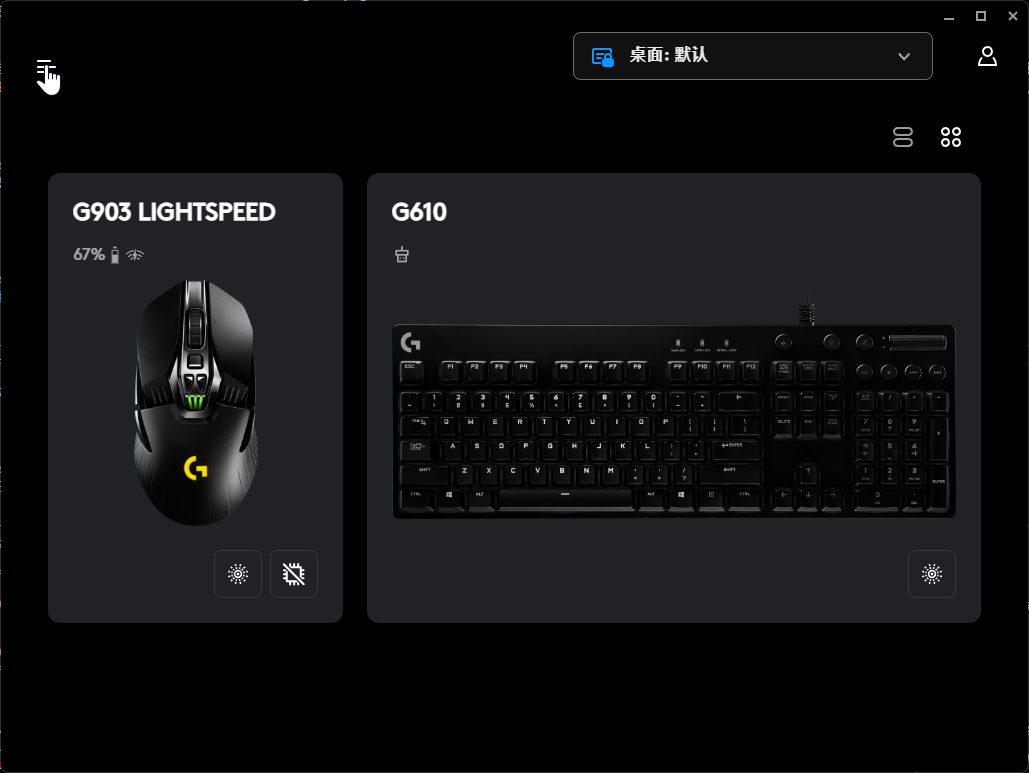
\includegraphics[width=\textwidth]{docs/assets/lghub_menu.png}
    \caption{展开左上角菜单}
\end{figure}

\begin{figure}[H]
    \Centering
    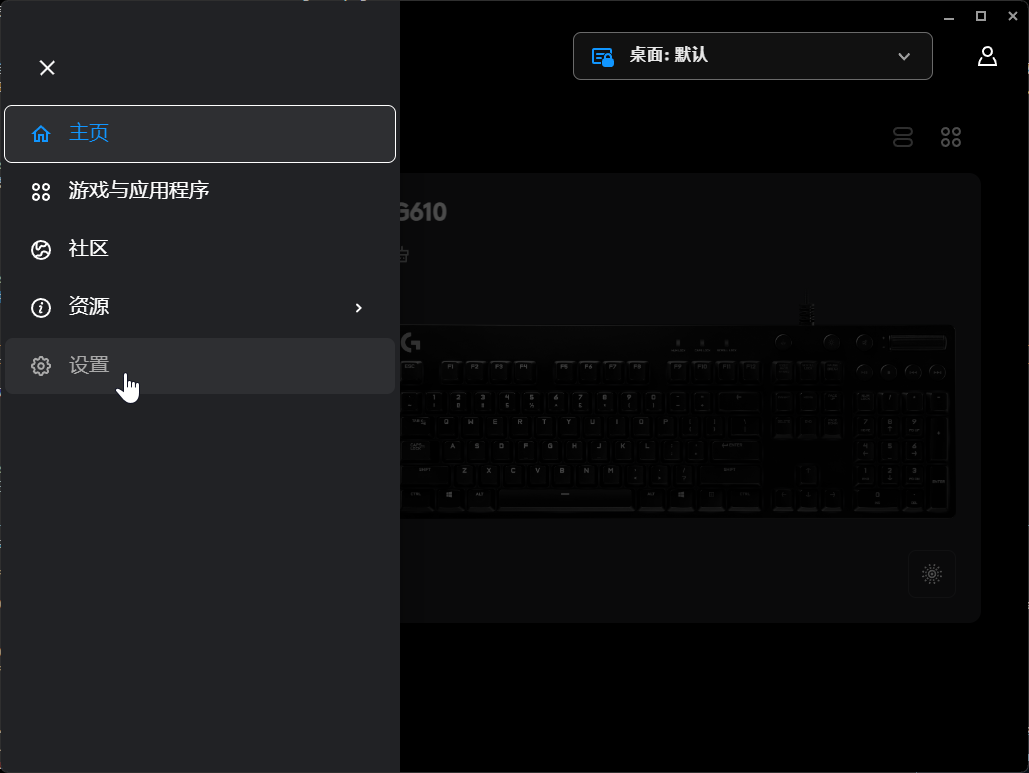
\includegraphics[width=\textwidth]{docs/assets/lghub_setting.png}
    \caption{点击“设置”}
\end{figure}

\begin{figure}[H]
    \Centering
    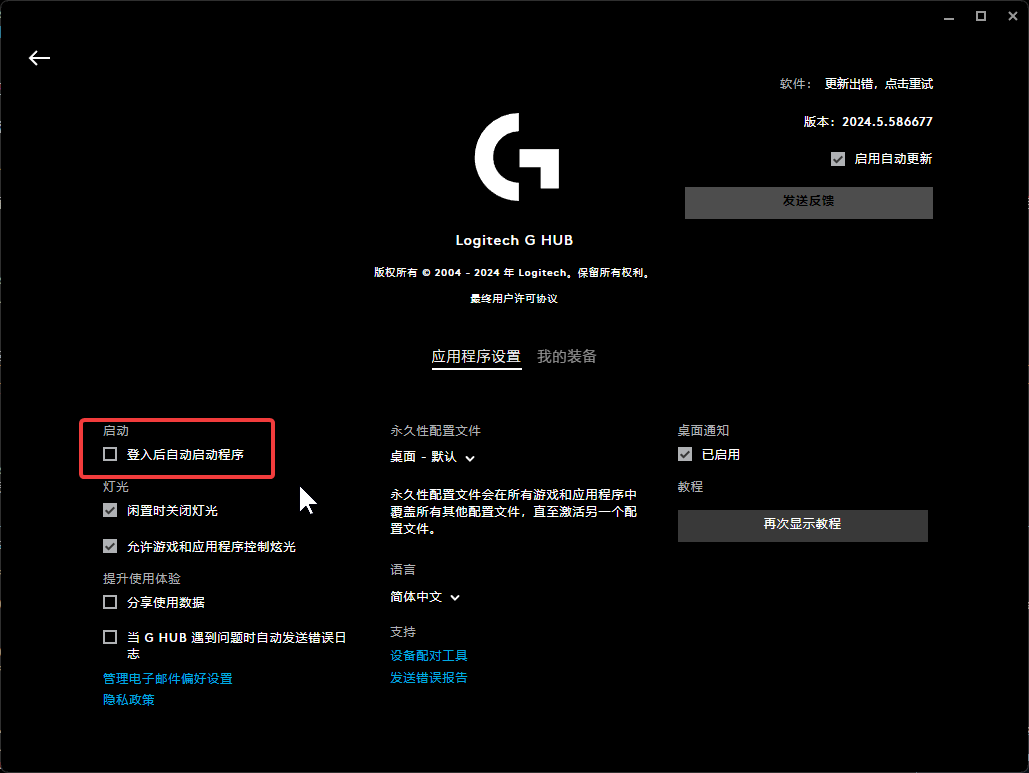
\includegraphics[width=\textwidth]{docs/assets/disable_login_start.png}
    \caption{关闭软件自启}
\end{figure}

返回到主界面,点击软件上方下拉框,选择“管理配置文件”。

\begin{figure}[H]
    \Centering
    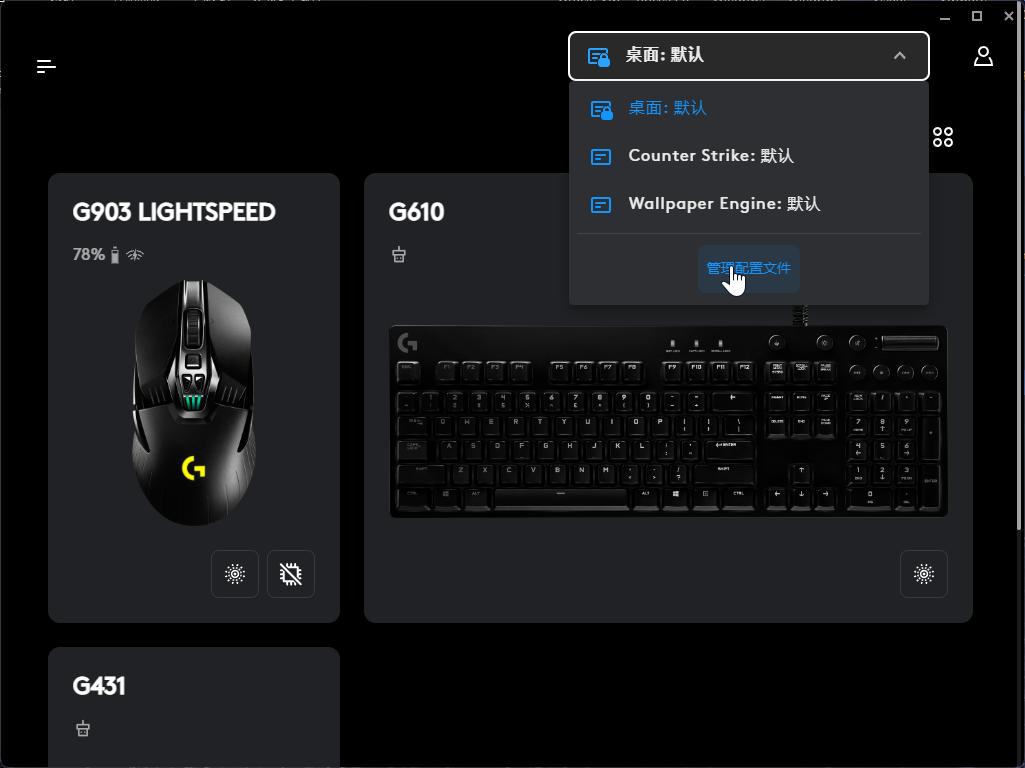
\includegraphics[width=\textwidth]{docs/assets/manage_configs.png}
    \caption{点击“管理配置文件”}
\end{figure}

在下一级界面中点击“编写脚本”。

\begin{figure}[H]
    \Centering
    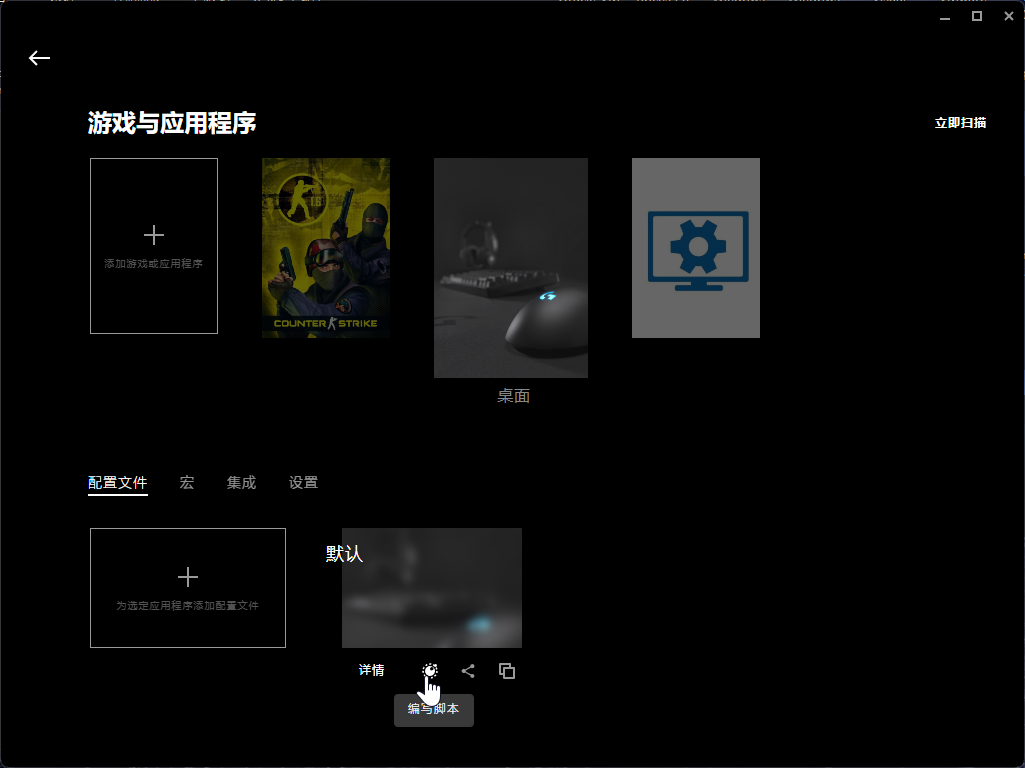
\includegraphics[width=\textwidth]{docs/assets/script.png}
    \caption{点击“编写脚本”}
\end{figure}

点击“脚本-导入”,将 LUA 源文件 \lstinline{main.lua} 导入软件,点击保存并运行。

\begin{figure}[H]
    \Centering
    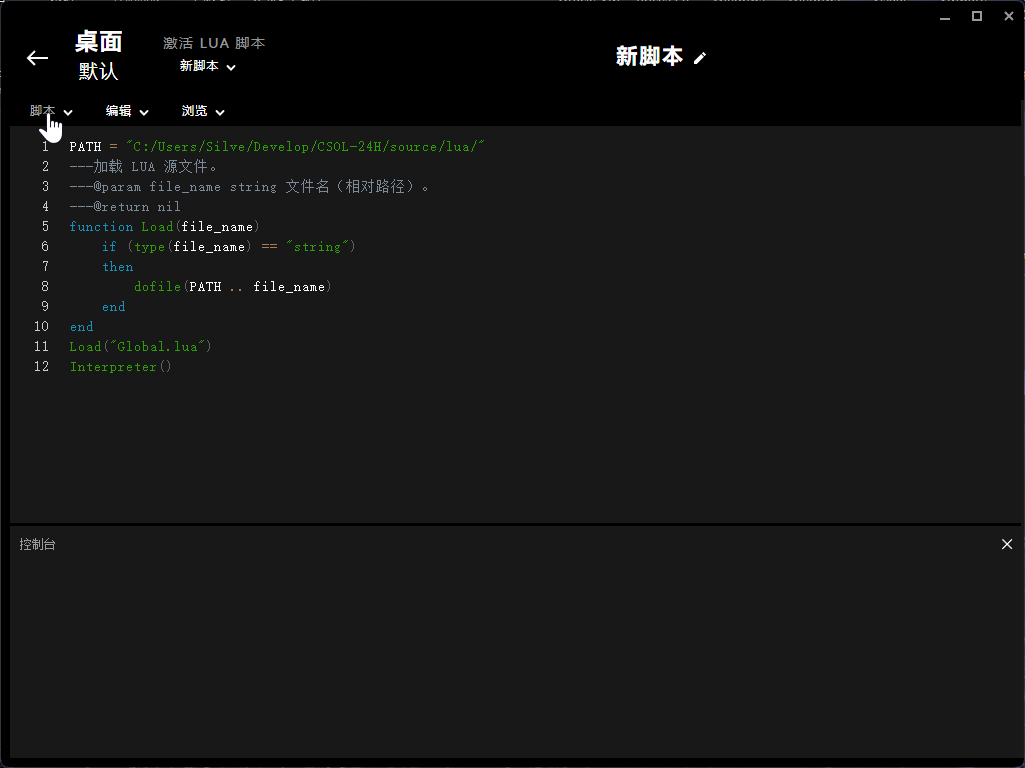
\includegraphics[width=\textwidth]{docs/assets/edit.png}
    \caption{点击“脚本”}
\end{figure}

\begin{figure}[H]
    \Centering
    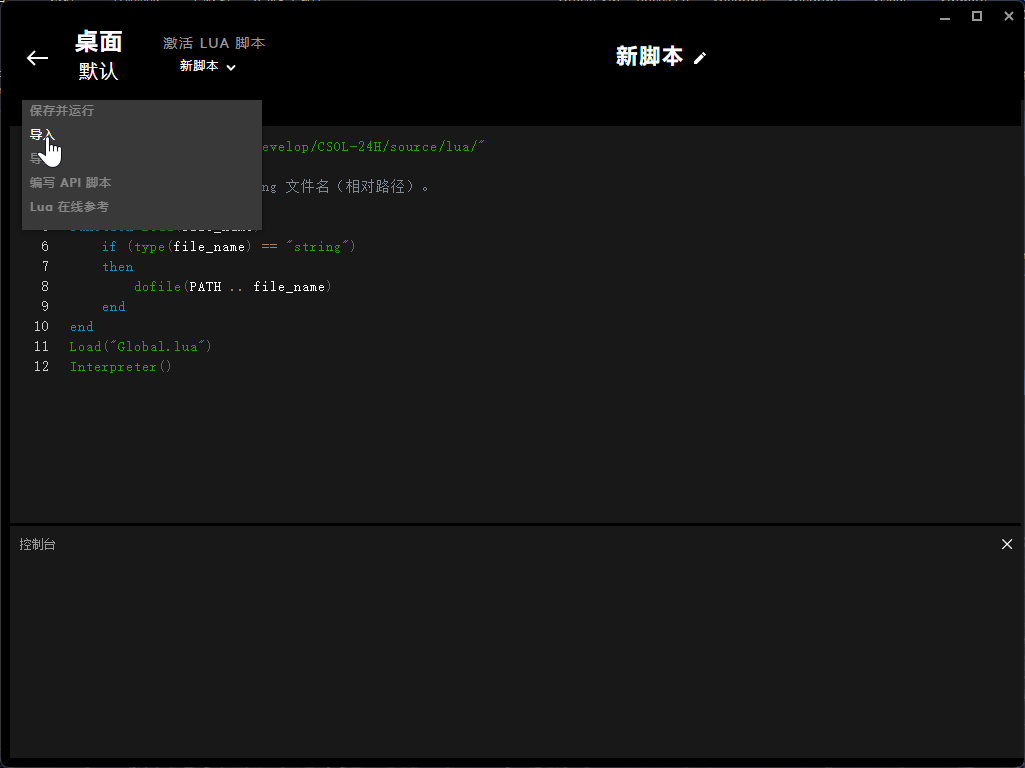
\includegraphics[width=\textwidth]{docs/assets/import.png}
    \caption{点击“导入”}
\end{figure}

\begin{figure}[H]
    \Centering
    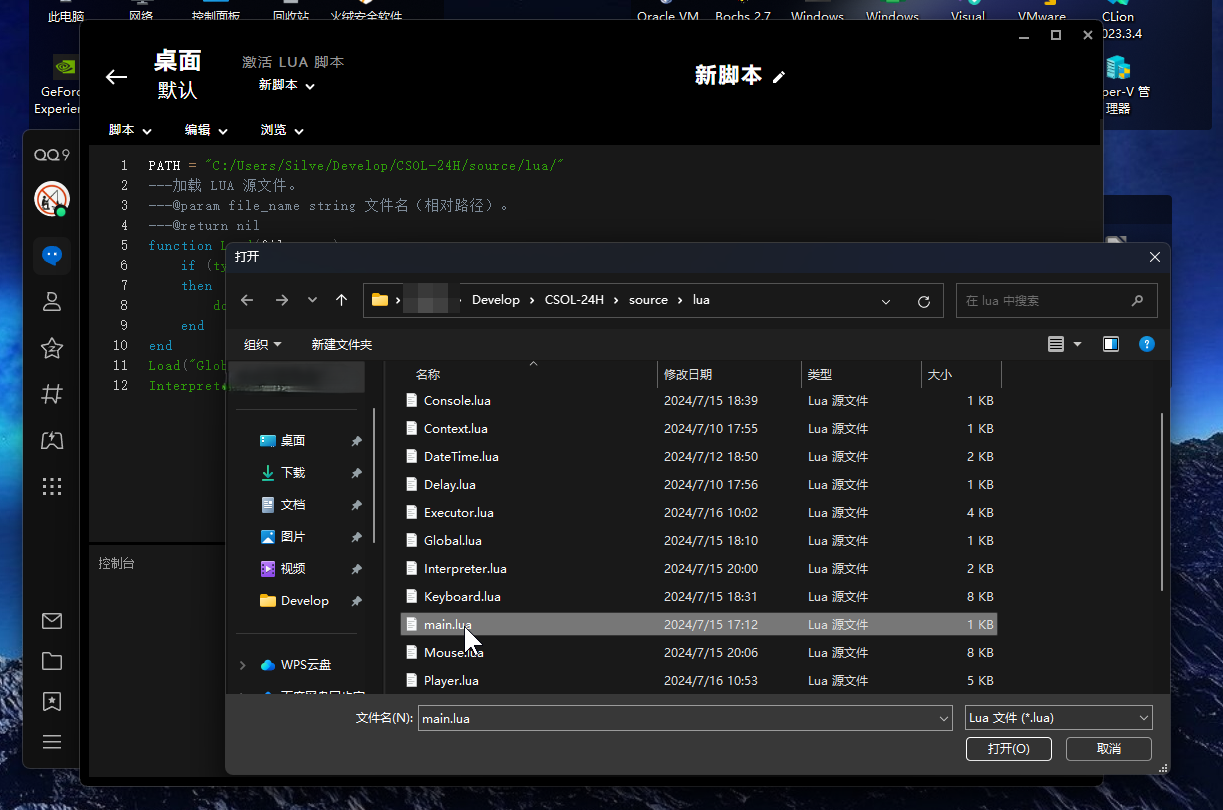
\includegraphics[width=\textwidth]{docs/assets/main.png}
    \caption{选择 \lstinline{main.lua}}
\end{figure}

\begin{figure}[H]
    \Centering
    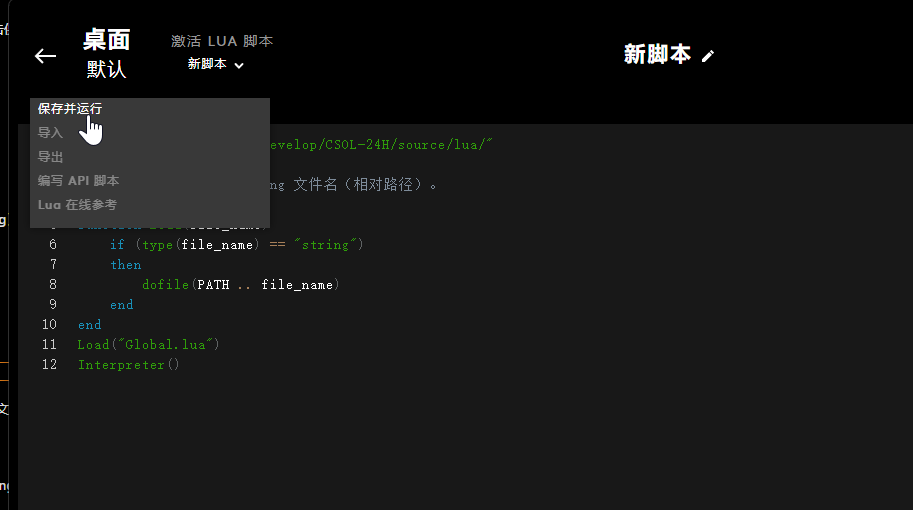
\includegraphics[width=\textwidth]{docs/assets/save_and_run.png}
    \caption{保存并运行}
\end{figure}

看到控制台输出下述文字信息,则说明导入成功。

\begin{figure}[H]
    \Centering
    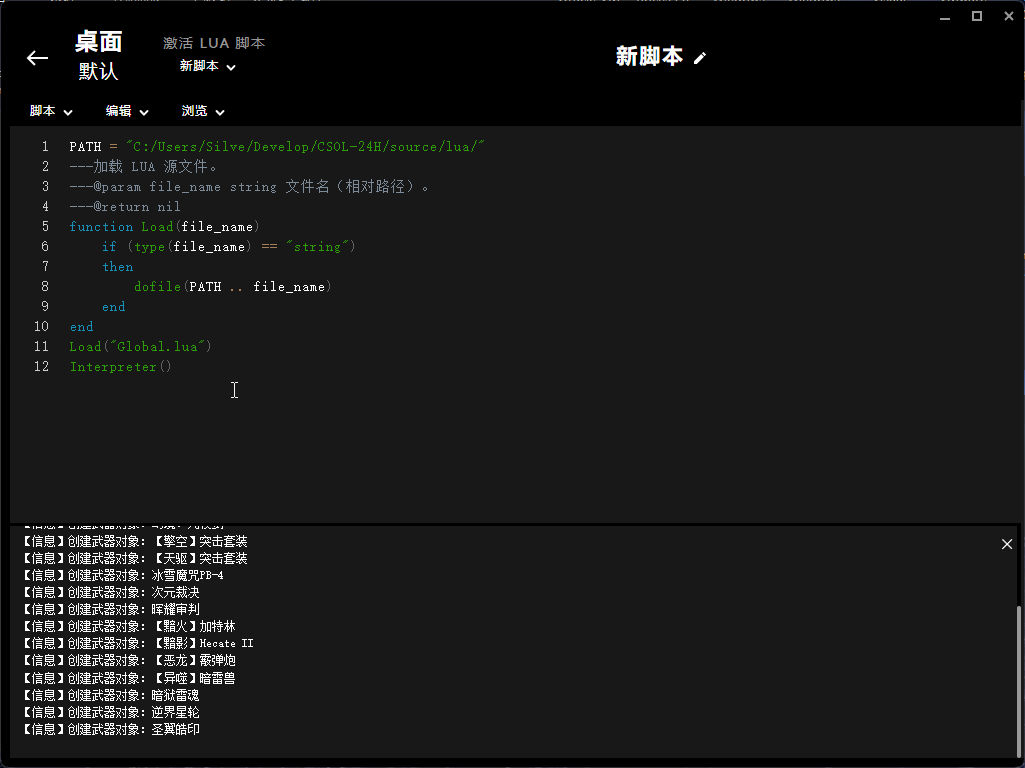
\includegraphics[width=\textwidth]{docs/assets/success.png}
    \caption{保存并运行成功}
\end{figure}

保存并运行后,罗技软件在下一次启动时会自动加载上述脚本文件(启动时加载只会执行一次),无需再重复上述操作。

\textbf{\color{red}但是,加载后若对文件夹内的任一个源文件进行修改,则还需要重新在此界面中保存运行。}

\subsection{控制器}

右键在 Powershell 中运行 \lstinline{Controller.ps1},控制器将启动。

\begin{figure}[H]
    \Centering
    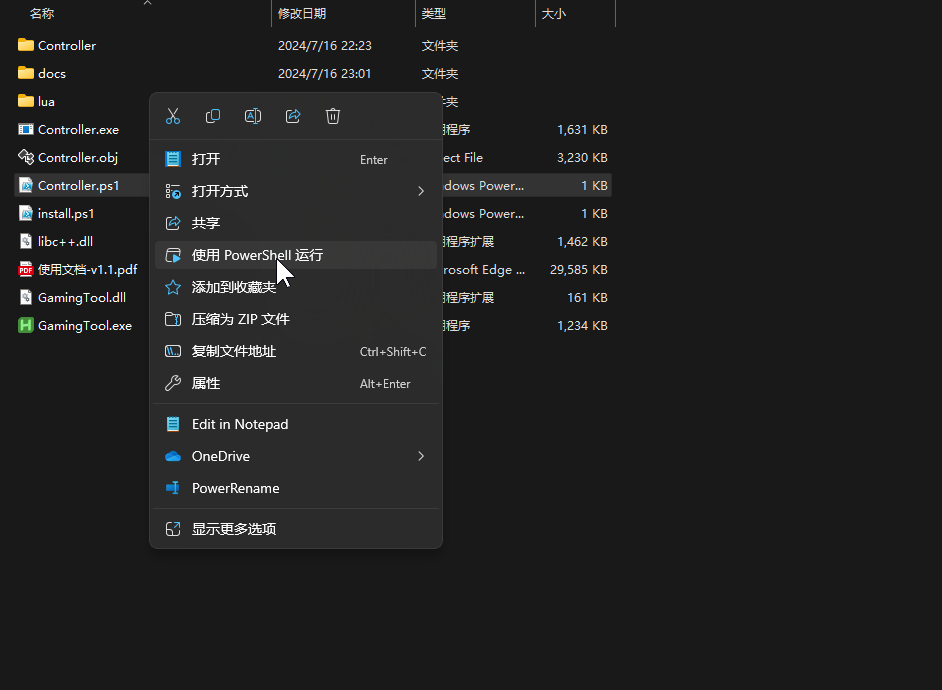
\includegraphics[width=\textwidth]{docs/assets/run_controller.png}
    \caption{运行控制器}
\end{figure}

控制器在 Windows 控制台中运行,在控制台界面中按下 \lstinline{Ctrl} \lstinline{C}(推荐)或直接点击右上角关闭按钮可终止程序。

启动控制器后,会注册如下热键(在阅读完本节之前请先不要尝试):

\begin{itemize}

    \item 0 模式:\lstinline{Ctrl} \lstinline{Alt} \lstinline{Shift} \lstinline{0},启动后的默认模式,该模式下不进行任何操作。

    \item 1 模式:\lstinline{Ctrl} \lstinline{Alt} \lstinline{Shift} \lstinline{1},单武器挂机模式。

    \item 2 模式:\lstinline{Ctrl} \lstinline{Alt} \lstinline{Shift} \lstinline{2},随机武器挂机模式。

    \item 3 模式:\lstinline{Ctrl} \lstinline{Alt} \lstinline{Shift} \lstinline{3},自动合成配件。

    \item 4 模式:\lstinline{Ctrl} \lstinline{Alt} \lstinline{Shift} \lstinline{4},自动重复购买同一件商店物品,可用于批量购买金币道具。

    \item 5 模式:\lstinline{Ctrl} \lstinline{Alt} \lstinline{Shift} \lstinline{5},定位坐标,将结果输出到罗技控制台。

\end{itemize}

控制器会在 \lstinline{lua} 目录下创建临时文件,实时向该临时文件中写入命令,指导 LUA 模块执行相应的操作。
每条命令都有一定的有效期(2 秒),超过有效期的命令不会被 LUA 模块执行。
每条命令的执行完毕都需要一定的时间,\textbf{\color{red}控制器切换模式不会立即停止当前命令的执行,而是有一定的延迟时间}。

\subsection{即时中断功能}

上面提到,控制器切换模式,LUA 模块响应有一定的延迟。
为了使罗技软件能够及时响应紧急的中断消息,本集成工具通过封装罗技 API,在 LUA 模块中引入了即时中断功能。

例如,\textbf{\color{red}若不慎错误地按下前面提及的功能热键,导致鼠标键盘不受控制,可以同时按下键盘上的左 \lstinline{Ctrl} 和右 \lstinline{Ctrl} 紧急暂停,罗技软件会在 10 毫秒内快速响应此中断信号。
紧急暂停后,罗技软件将不再发出任何键鼠操作,直至同时按下键盘上的左 \lstinline{Alt} 和右 \lstinline{Alt} 恢复。}

相应地,您可以在罗技软件控制台中看到相应的提示信息。

\begin{figure}[H]
    \Centering
    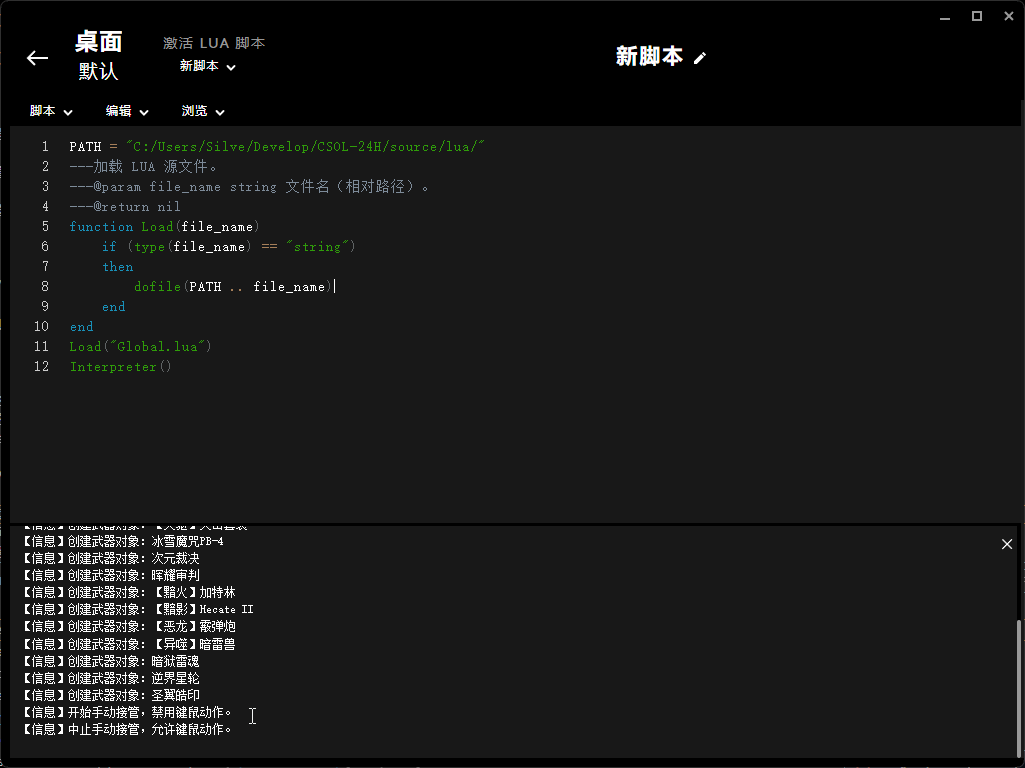
\includegraphics[width=\textwidth]{docs/assets/interrupt.png}
    \caption{即时中断功能提示信息}
\end{figure}

需要注意,紧急暂停功能完全独立于控制器。
\textbf{\color{red}紧急暂停后,控制器仍然会持续向罗技软件下达命令,只是罗技软件并不会执行这些命令。}若要取消当前控制器启用的模式,请按热键将控制器切换回 0 模式。

\subsection{使用 GamingTool}

双击运行解压目录下的 \lstinline{GamingTool.exe}。

有关 GamingTool 使用方法,参考 \href{https://gitee.com/silver1867/gaming-tool}{GamingTool 项目链接}。

\subsection{配置文件}

\textbf{\color{red}\lstinline{lua} 目录下的 \lstinline{Setting.lua} 及 \lstinline{WeaponList.lua} 是根据用户自身情况自行定义的配置文件。
按照本文档介绍的方式配置完毕能够正常使用后,您应当妥善保管。后续版本更新不会对这两个配置文件内容作出较大的变动。当您修改配置文件内容后,必须在罗技软件中重新导入并保存运行。}
